\documentclass{article}

% Language setting
% Replace `english' with e.g. `spanish' to change the document language
\usepackage[english]{babel}
\usepackage{indentfirst}

% Set page size and margins
% Replace `letterpaper' with `a4paper' for UK/EU standard size
\usepackage[letterpaper,top=2cm,bottom=2cm,left=3cm,right=3cm,marginparwidth=1.75cm]{geometry}

% Useful packages
\usepackage{amsmath}
\usepackage{graphicx}
\usepackage[colorlinks=true, allcolors=blue]{hyperref}

\title{Supplementary Material}
\date{} 
\begin{document}
\maketitle
% In this supplemental material, we provide more experimental results with different cases. 

% \section{Results with no explicit regularization}
% DC resistivity inversion is very ill-posed in many cases; therefore, we need to have explicit regularization terms to recover a realistic subsurface map. In this section, we show the inversion results with no or less regularization terms to verify this statement. Note that it has been found that in certain scenarios, the smallness and reference model are not necessary in DC resistivity inversion\textcolor{red}{\cite{}}, but it's not true in the scenarios of our study cases.

% \subsection{Inversion results with no smallness and smoothness term}

% \subsection{Inversion results with only smoothness term}

% With all conventional inversion results shown above, we conclude that the smallness term is necessary n in the chosen survey configuration and subsurface structures of this study. 

\section{Results with different noise level}

We choose the inversions with $5\%$ Gaussian noise in the main manuscript. Here we show the inversion results with different noise levels.

For seismic inversions such as full-waveform inversion or seismic tomography inversion, high-level noise will produce high-frequency artifacts on the inversion results without corrupting the recovery of the main targets. The physics governing the DCR method and seismic methods are very different (Poisson’s equation and wave equation). Unlike the seismic methods, the high-level noise will corrupt the recovery of the main targets in DCR inversion results in both the conventional inversions and DIP-Inv. 

\subsection{Inversion results with larger noise}
This subsection presents the inversion results from DIP-Inv with $10\%$ Gaussian noise. Figure \ref{fig_1} shows (a) the true model, (b) the conventional sparse-norm result without sensitivity weighting, (c) the conventional sparse-norm results with sensitivity weighting and (d) the DIP-Inv results. When the noise level is higher, the regularization has a larger influence as compared to the results shown in Figures 6 and 7 of the main manuscript. That is because we include the uncertainties in our construction of the data misfit term. As a result, it is not unexpected that the recovered models do not characterize the extension of the dipping target. 

The conventional inversion without sensitivity has unwanted near-electrodes artifacts [Fig. \ref{fig_1}(b)] as discussed in section II A in the main manuscript. Adding sensitivity weighting in the conventional inversion eliminates these artifacts but poorly resolves the top layer [Fig. \ref{fig_1}(c)]. In comparing each of the results, we still see that the DIP-Inv result [Fig. \ref{fig_1}(d)] does the best in terms of recovering a compact target with the correct dip and better recovery of the top layer. To further evaluate [Fig. \ref{fig_1}(c)] and [Fig. \ref{fig_1}(d)], we present MAE and MSE results between the inversion results and the true models [Table \ref{table:1}]. From the table, you can see that our methods have better scores (lower values of MAE and MAE) in all three cases in the higher noise scenario. This supports our argument that in comparing each of the results, we still see that the DIP-Inv result does the best.  

\begin{figure}[h!]
\centering
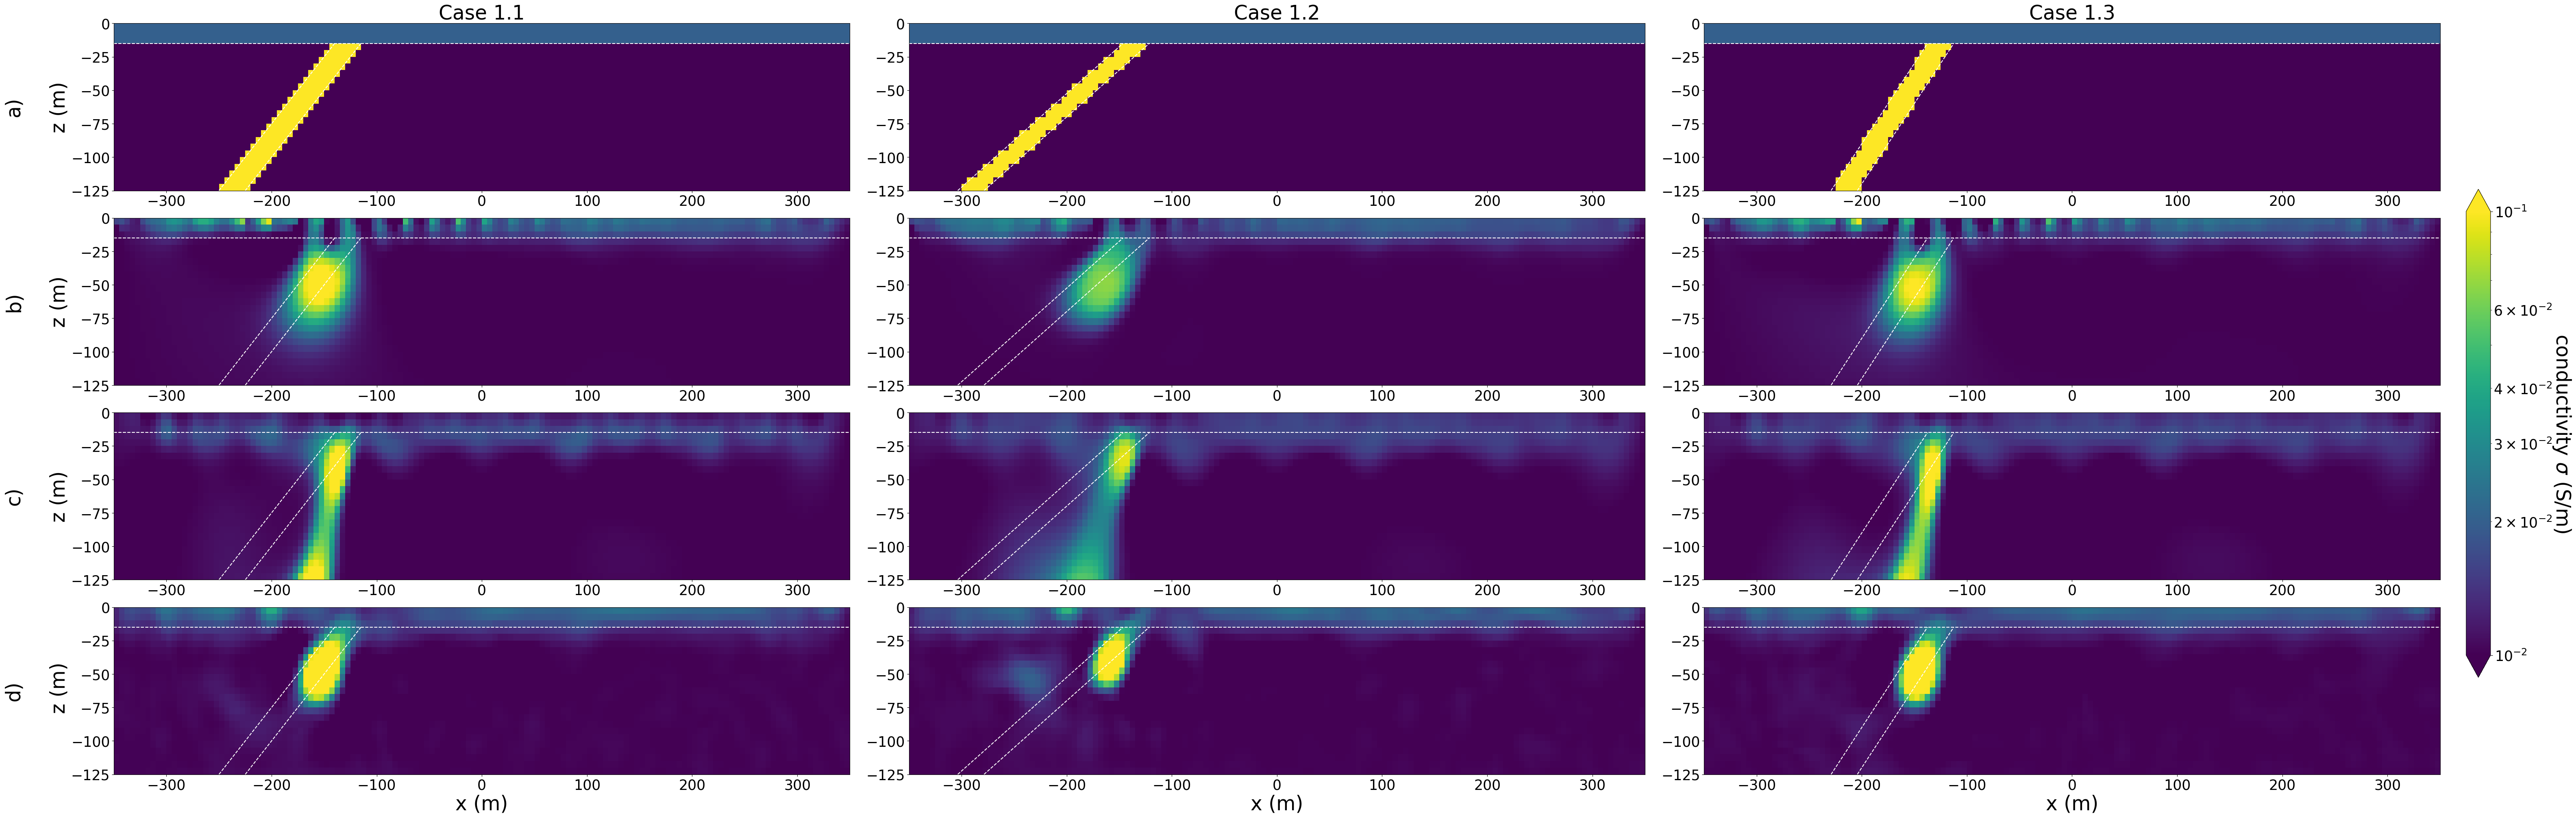
\includegraphics[width=1.\linewidth]{Figure_6_0.1.png}
\caption{(a) is the true model; the dip of the dike is varied. (b) and (c) are from the conventional sparse-norms inversions without/with sensitivity weighting respectively. (d) is the DIP-Inv result. All inversions are done in the scenarios that the observations have 10$\%$ Gaussian noise.}
\label{fig_1}
\end{figure}

\begin{table}[b!]
\centering
\caption{Comparison of DIP-Inv and the conventional method with sensitivity weighting in the scenarios of 10$\%$ noise}
\begin{tabular}{|c|c|l|l|}
\hline
Model & Metrics & Conventional method & DIP-Inv\\
\hline
Case 1.1 & MAE $\downarrow$ & 0.2153 & \textbf{0.1346}\\
 & MSE $\downarrow$ & 0.0065 & \textbf{0.0052}\\
\hline
Case 1.2 & MAE $\downarrow$ & 0.2237 & \textbf{0.1305}\\
 & MSE $\downarrow$ & 0.0058 & \textbf{0.0052}\\
\hline
Case 1.3 & MAE $\downarrow$ & 0.2194 & \textbf{0.1275}\\
 & MSE $\downarrow$ & 0.0062 & \textbf{0.0051}\\ 
\hline
\end{tabular}
\label{table:1}
\end{table}

\begin{figure}[h!]
\centering
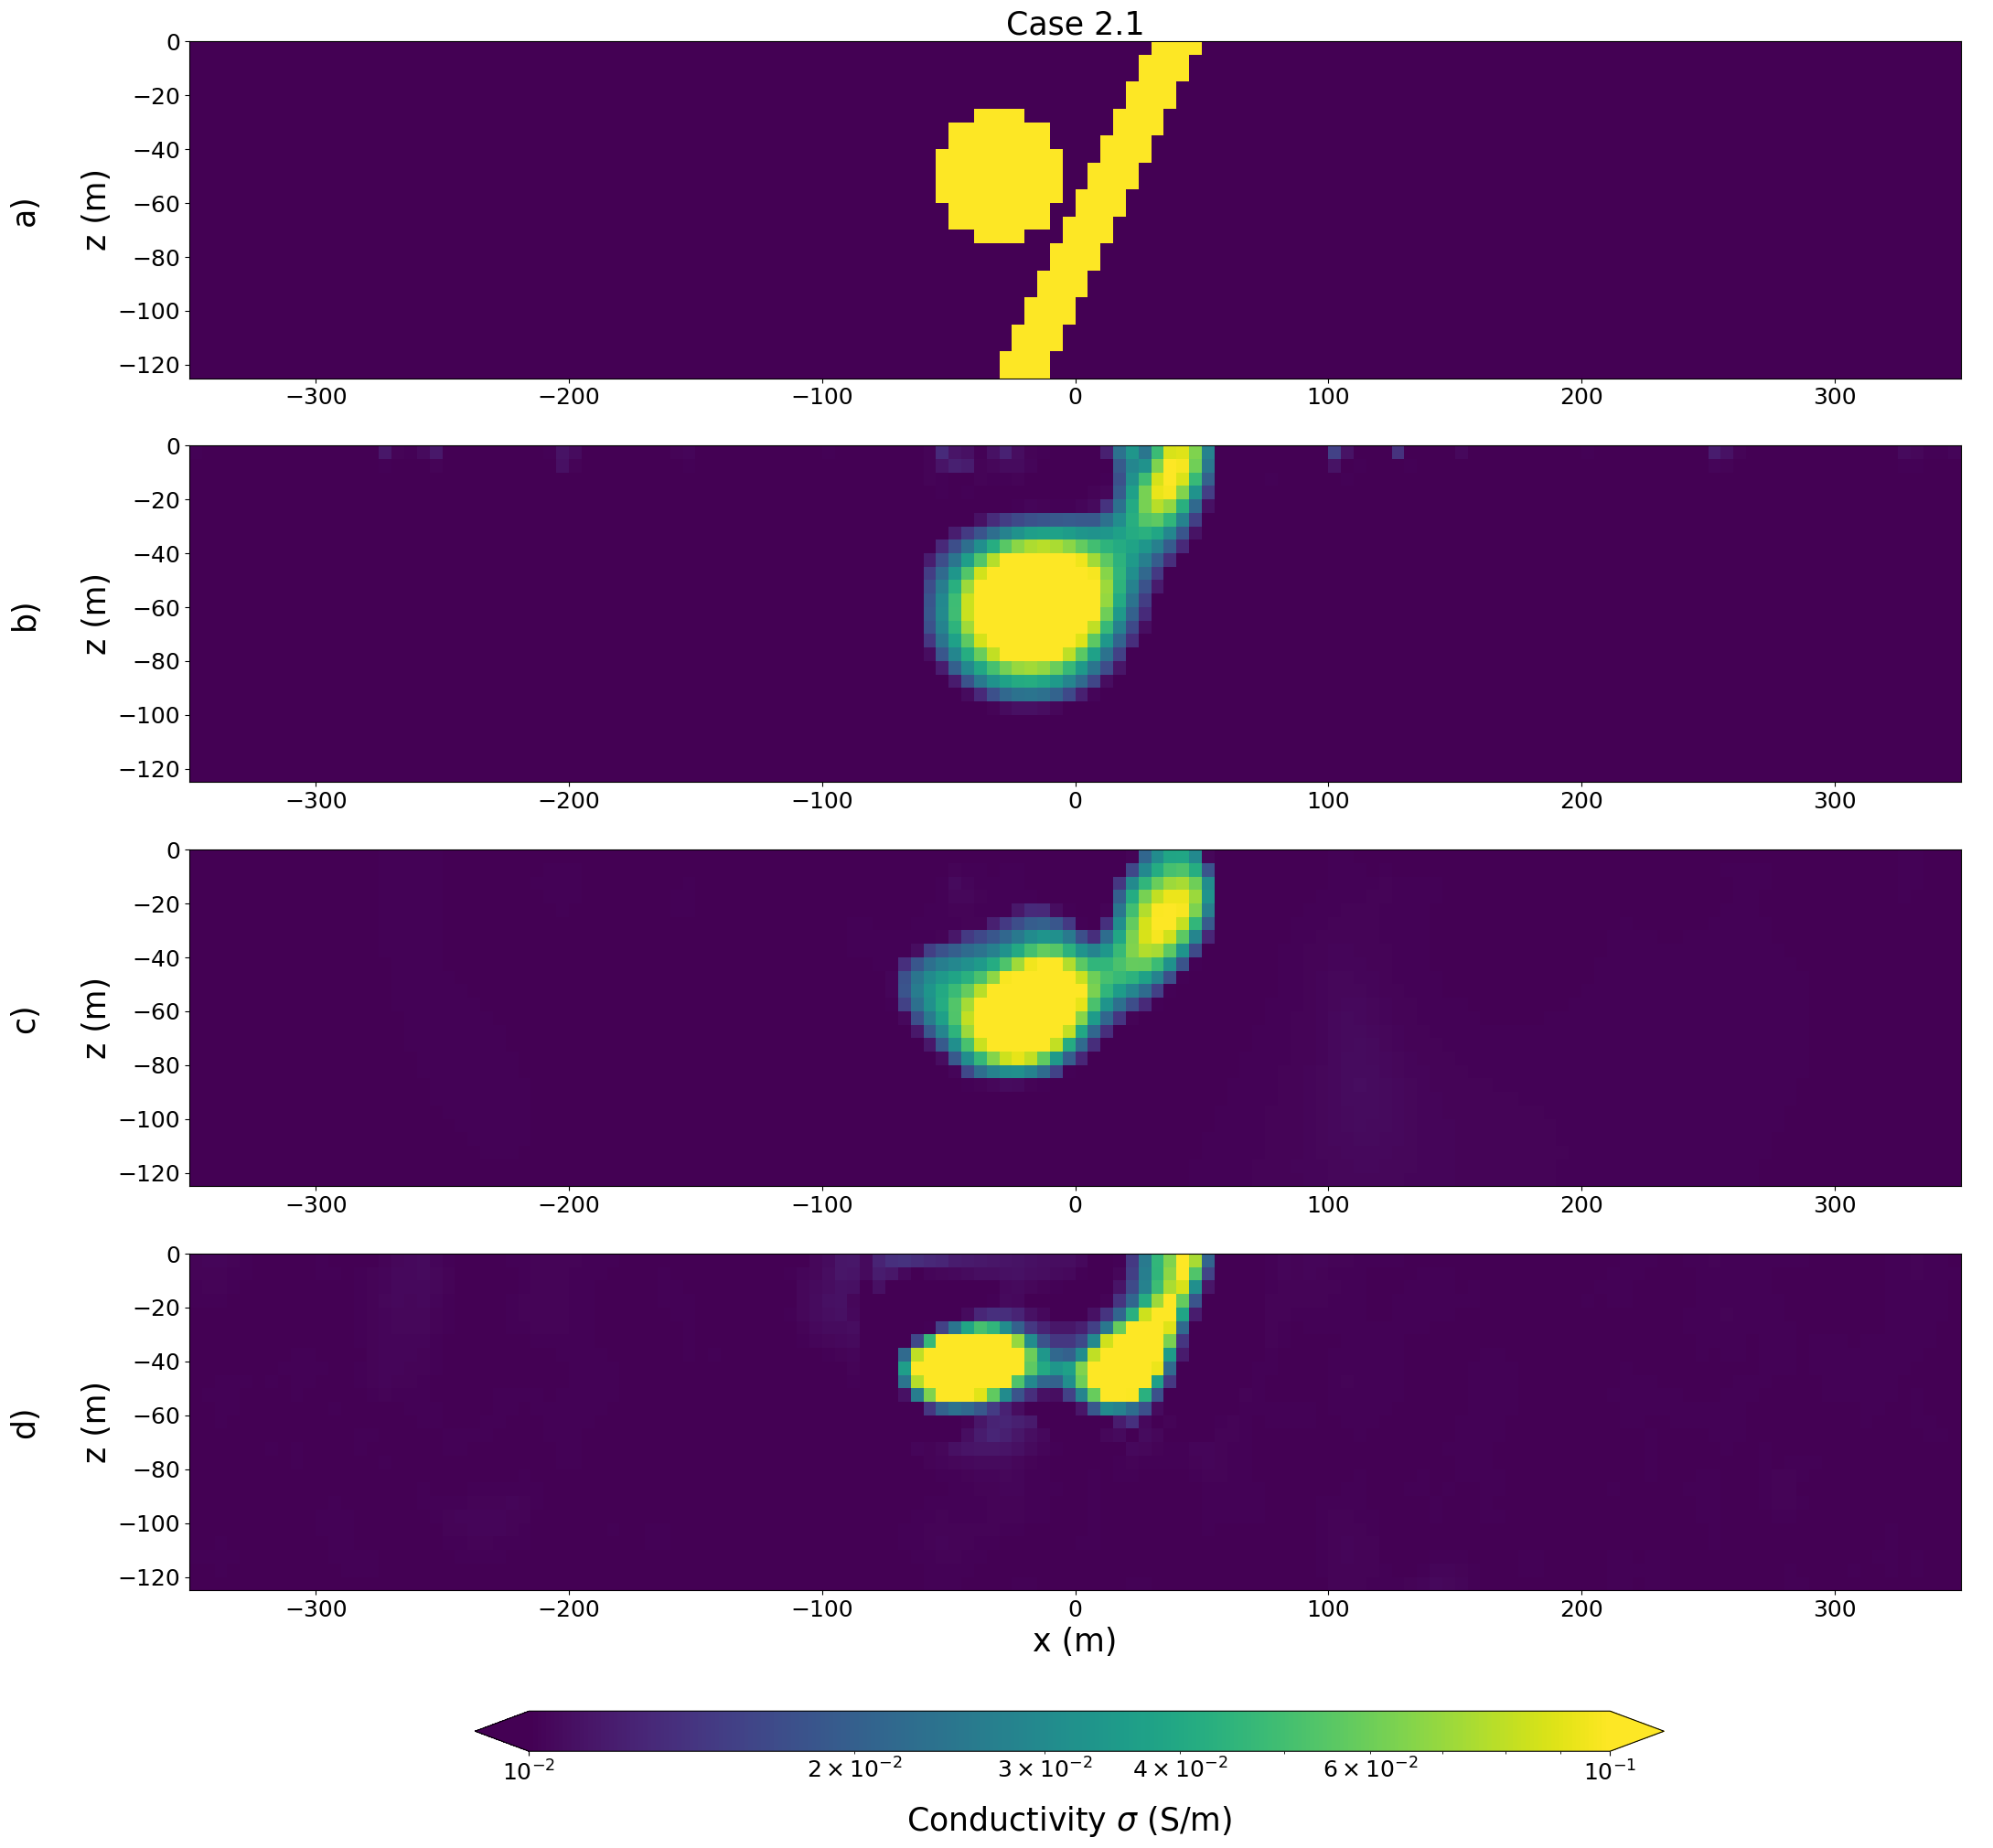
\includegraphics[width=.45\linewidth]{Figure_Case2.1_0.1.png}
\caption{(a) is the true model. (b) and (c) are from the conventional sparse-norms inversions without/with sensitivity weighting respectively. (d) is the DIP-Inv result. All inversions are done in the scenario that the observations have 10$\%$ Gaussian noise.}
\label{fig_2}
\end{figure} 


\begin{figure}[h!]
\centering
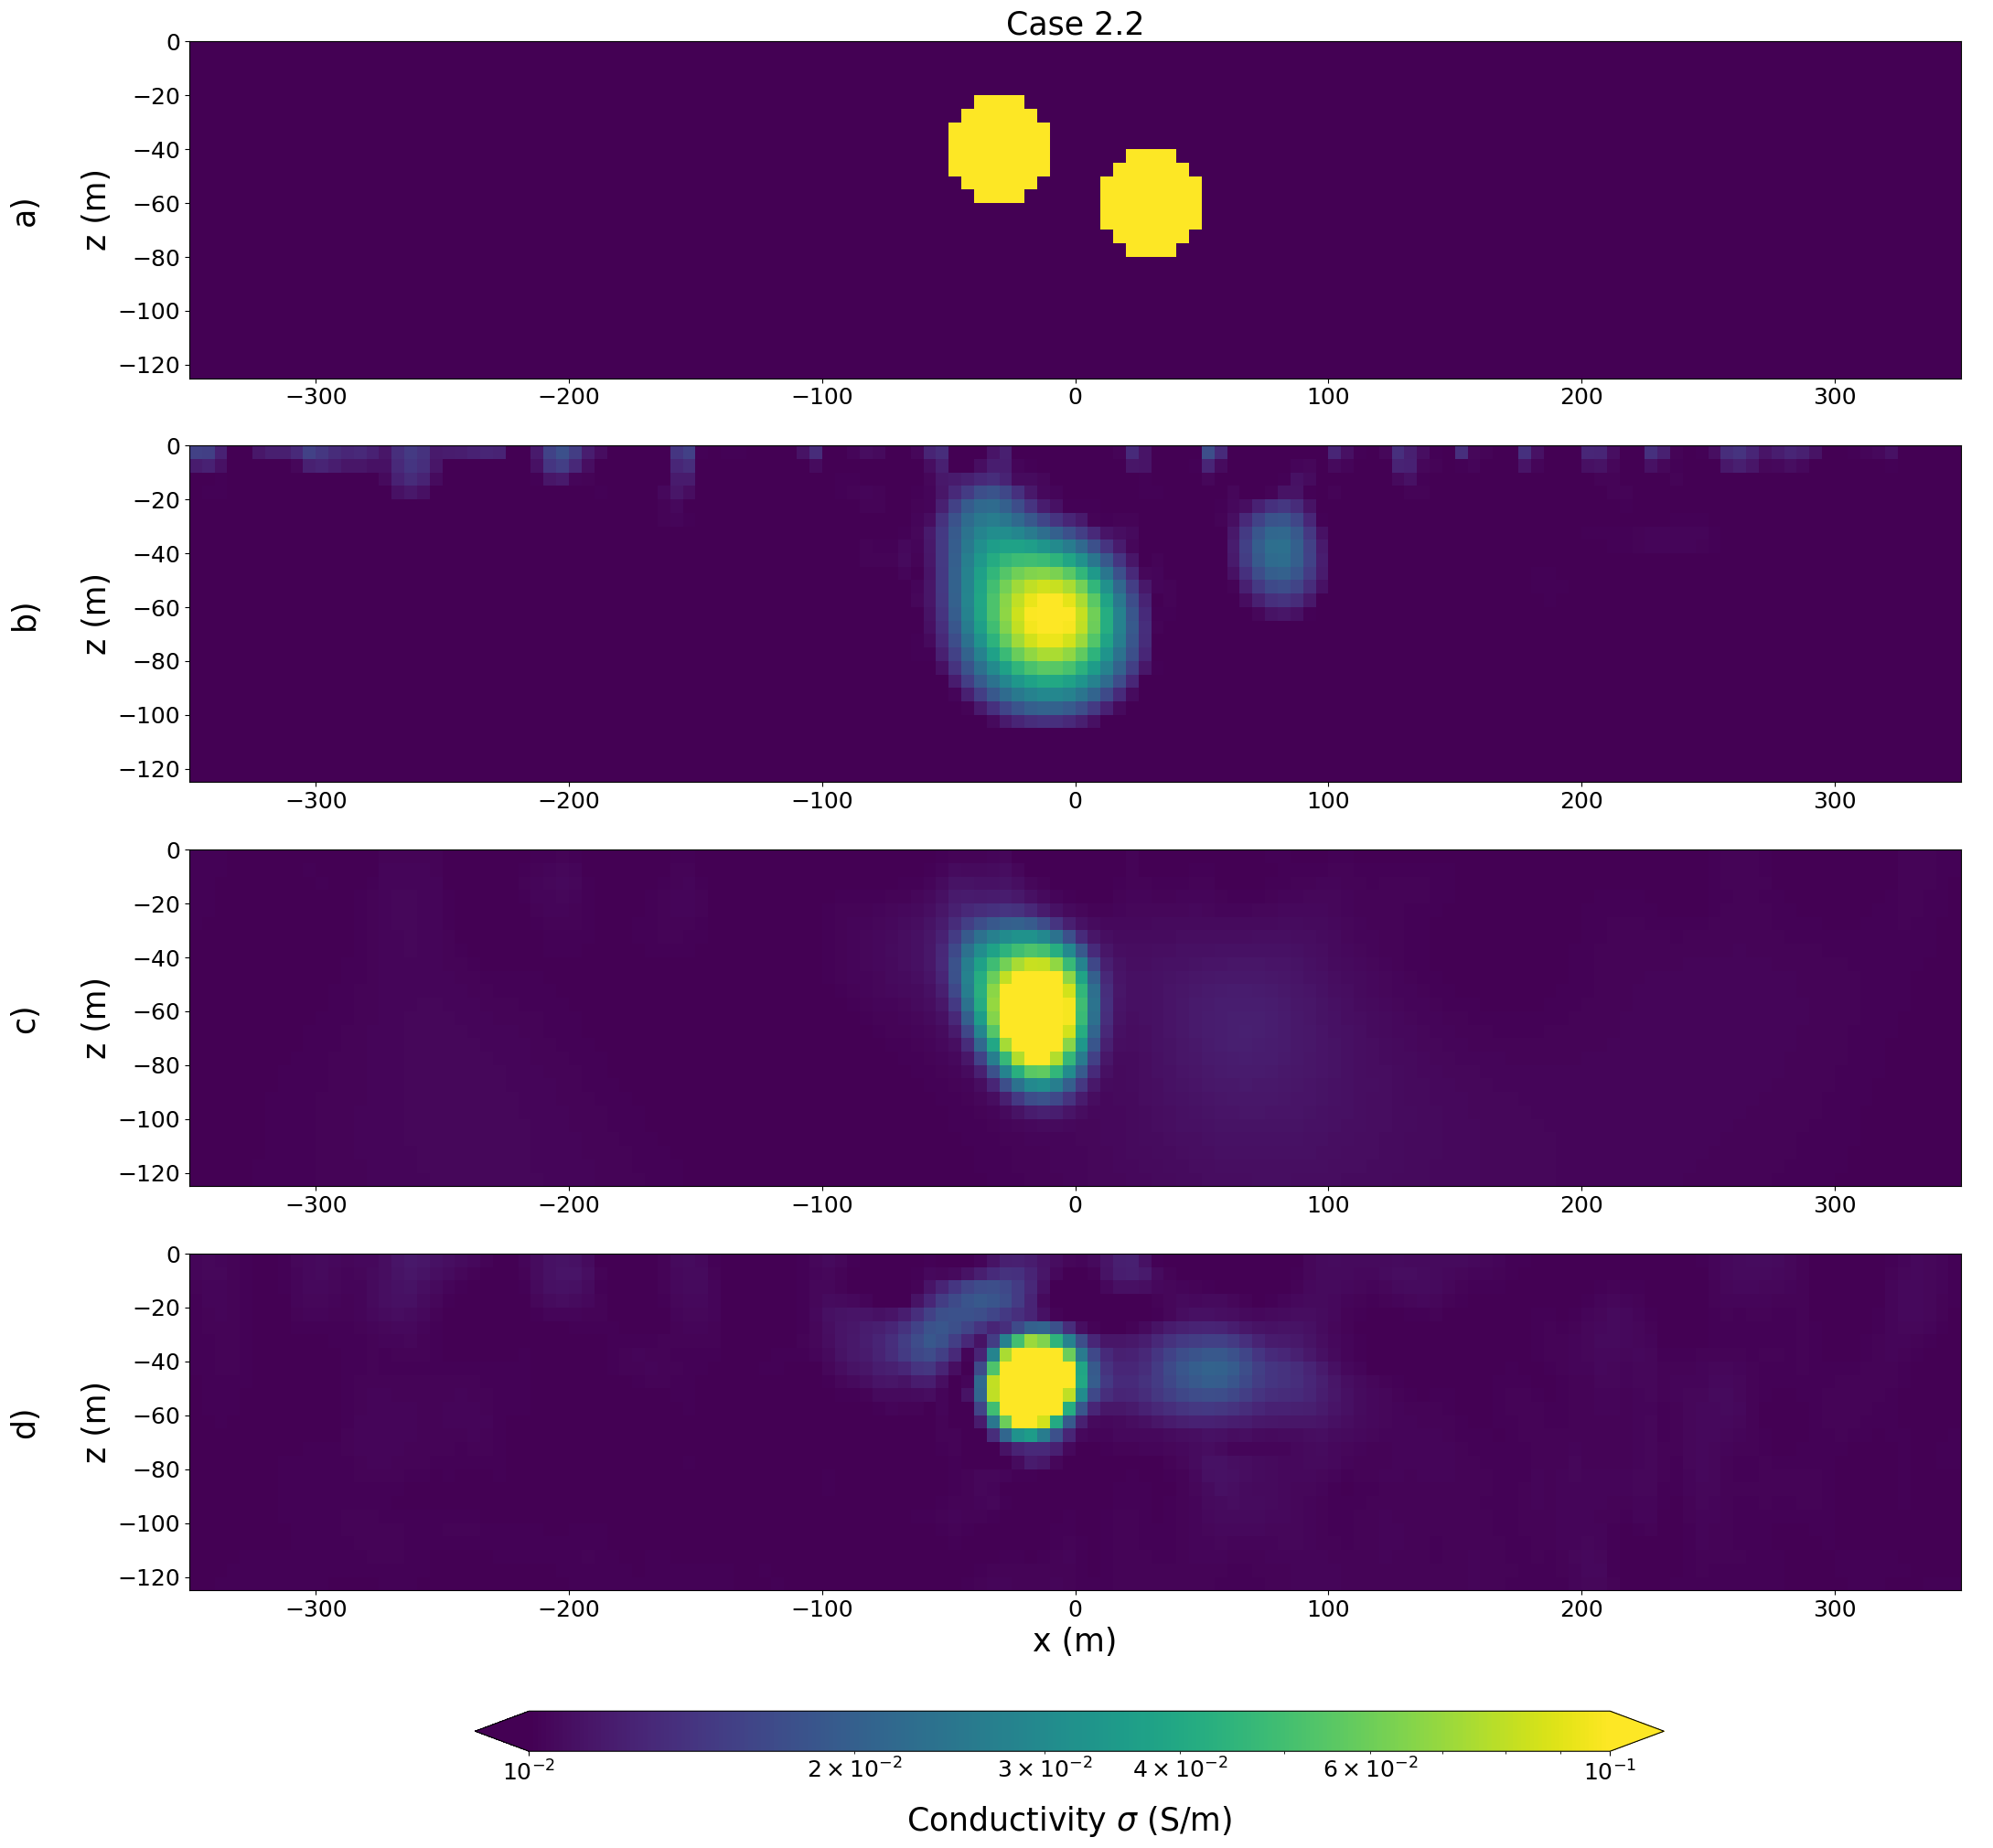
\includegraphics[width=.45\linewidth]{Figure_8_0.1.png}
\caption{(a) is the true model. (b) and (c) are from the conventional sparse-norms inversions without/with sensitivity weighting respectively. (d) is the DIP-Inv result. All inversions are done in the scenario that the observations have 10$\%$ Gaussian noise.}
\label{fig_3}
\end{figure}

We performed a similar analysis for Case 2 in a higher noise scenario as well. For Case 2.1, the cylindrical structure and the dike structure merge together in the conventional results [Fig. \ref{fig_2}(b) and (c)]. In contrast, the DIP-Inv [Fig. \ref{fig_2}(d)] is able to show the separation of the cylindrical structure and the dike structure, and the recovered structures are more compact than the conventional results. 
% Again, since more noise has been added, we see that in all results deeper structures are not resolved. 

For Case 2.2, the conventional inversion without sensitivity weighting [Fig. \ref{fig_3}(b)] has unwanted near-electrode artifacts. Adding sensitivity weighting eliminates these artifacts [Fig. \ref{fig_3}(c)]. All methods struggle to recover the the deeper cylindrical structure, because deeper structures will be more influenced by the large noise level. The DIP-Inv result produces a more compact, cylindrical target as compared to the conventional approaches. We further support the DIP-Inv result [Fig. \ref{fig_3}(d)] does the best by the MAE and MSE results shown in Table \ref{table:2}. From the table, you can see that our methods have better scores in both cases except for the MAE score of Case 2.1.

\begin{table}[h!]
\centering
\caption{Comparison of DIP-Inv and the conventional method with sensitivity weighting in the scenarios of 10$\%$ noise}
\begin{tabular}{|c|c|l|l|}
\hline
Model & Metrics & Conventional method& DIP-Inv\\
\hline
Case 2.1 & MAE $\downarrow$ & \textbf{0.0801} & 0.0881\\
 & MSE $\downarrow$ & 0.0049 & \textbf{0.0045}\\
\hline
Case 2.2 & MAE $\downarrow$ & 0.0901 & \textbf{0.0772}\\
 & MSE $\downarrow$ & 0.0049 & \textbf{0.0045}\\
\hline
\end{tabular}
\label{table:2}
\end{table}
\pagebreak
\subsection{Inversion results with less noise}
In this subsection, we present the inversion results with $3\%$ Gaussian noise. 

Fig. \ref{fig_4} shows the inversion results for Cases 1.1-1.3 when $3\%$ Gaussian noise is added to the data. For these examples, the dip angle is best recovered in the DIP-Inv results. Table \ref{table:3} shows the MAE and MSE scores for Cases 1.1-1.3, DIP-Inv inversion results have better perfermence in all three cases in terms of the score values. 

\begin{figure}[h!]
\centering
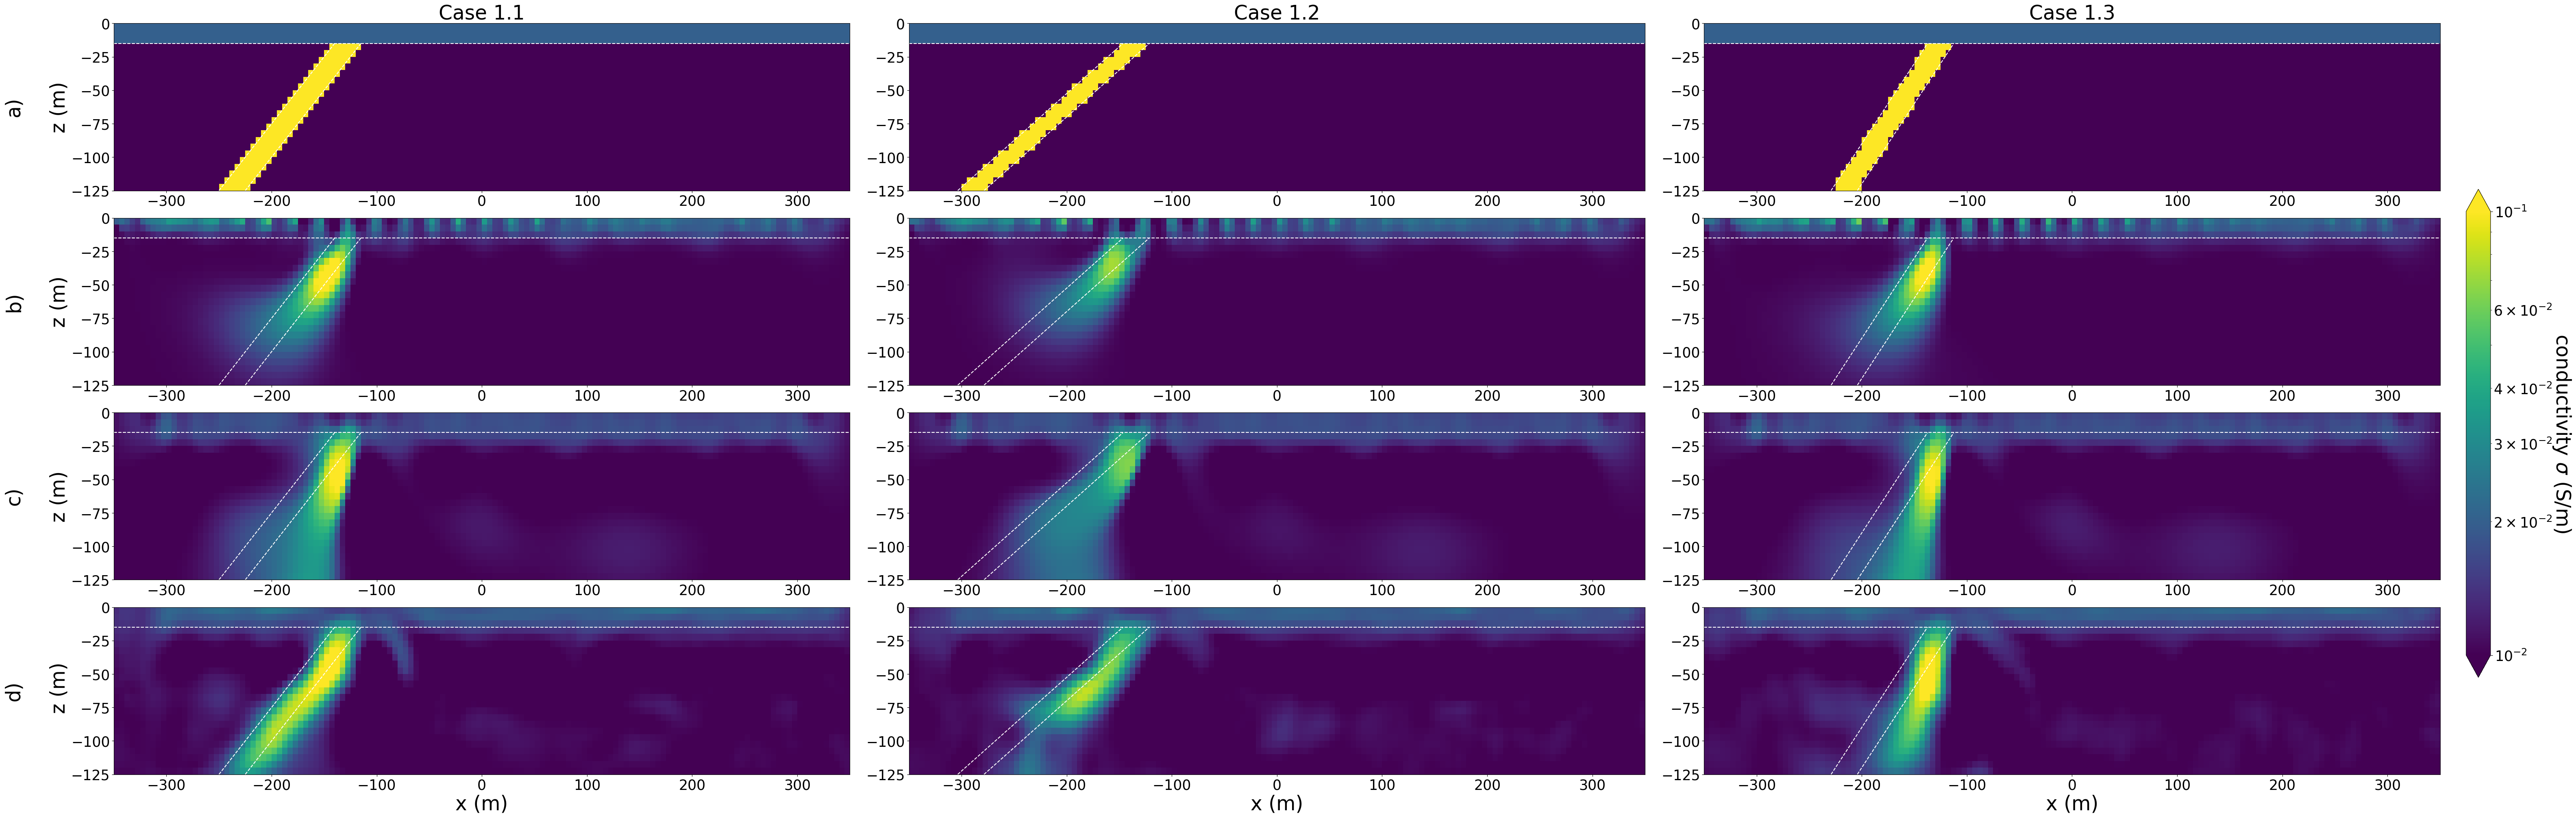
\includegraphics[width=1\linewidth]{Figure_6_0.03.png}
\caption{(a) is the true model; the dip of the dike is varied. (b) and (c) are from the conventional sparse-norms inversions without/with sensitivity weighting respectively. (d) is the DIP-Inv result. All inversions are done in the scenarios that the observations have 3$\%$ Gaussian noise.}
\label{fig_4}
\end{figure}

\begin{table}[b!]
\centering
\caption{Comparison of DIP-Inv and the conventional method with sensitivity weighting in the scenarios of 3$\%$ noise}
\begin{tabular}{|c|c|l|l|}
\hline
Model & Metrics & Conventional method & DIP-Inv\\
\hline
Case 1.1 & MAE $\downarrow$ & 0.2180 & \textbf{0.1550}\\
 & MSE $\downarrow$ & 0.0057 & \textbf{0.0045}\\
\hline
Case 1.2 & MAE $\downarrow$ & 0.2123 & \textbf{0.1694}\\
 & MSE $\downarrow$ & 0.0054 & \textbf{0.0051}\\
\hline
Case 1.3 & MAE $\downarrow$ & 0.2182 & \textbf{0.1805}\\
 & MSE $\downarrow$ & 0.0057 & \textbf{0.0055}\\ 
\hline
\end{tabular}
\label{table:3}
\end{table}

The results for Cases 2.1 and 2.2 are shown in Figures \ref{fig_5} and \ref{fig_6}, respectively. For Case 2.1, the conventional results [Fig. \ref{fig_5}(b) and (c)] merge the cylindrical structure and the dike structure together and diverge in the deeper depth, but the DIP-Inv result [Fig. \ref{fig_5}(d)] is able to recover the right shape of the two structures. For Case 2.2, both the inversions from the conventional method with sensitivity weighting [Fig. \ref{fig_5}(c)] and DIP-Inv [Fig. \ref{fig_5}(d)] perform well in detecting two cylindrical structures. Table \ref{table:4} show the MAE and MSE scores for Case 2.1 and Case 2.2. From the scores, we can see that DIP-Inv shows an improvement above the conventional results in most cases. The DIP-Inv result is inferior to the conventional result in Case 2.2. 
There are multiple choices that need to be made when implementing the DIP-Inv approach, including, for example, the number of hidden layers in the CNN, the learning rate, and the cooling strategy used, as discussed in Section IV in the main manuscript. We used the same hyperparameters for the inversions in the scenario of 3$\%$ noise as in the scenario of 5$\%$ noise to illustrate the robustness of DIP-Inv. However, in practice, we would recommend that multiple architectures be tested so that the hyperparameters chosen appropriately match the noise level and complexity of the model.


\begin{figure}[h!]
\centering
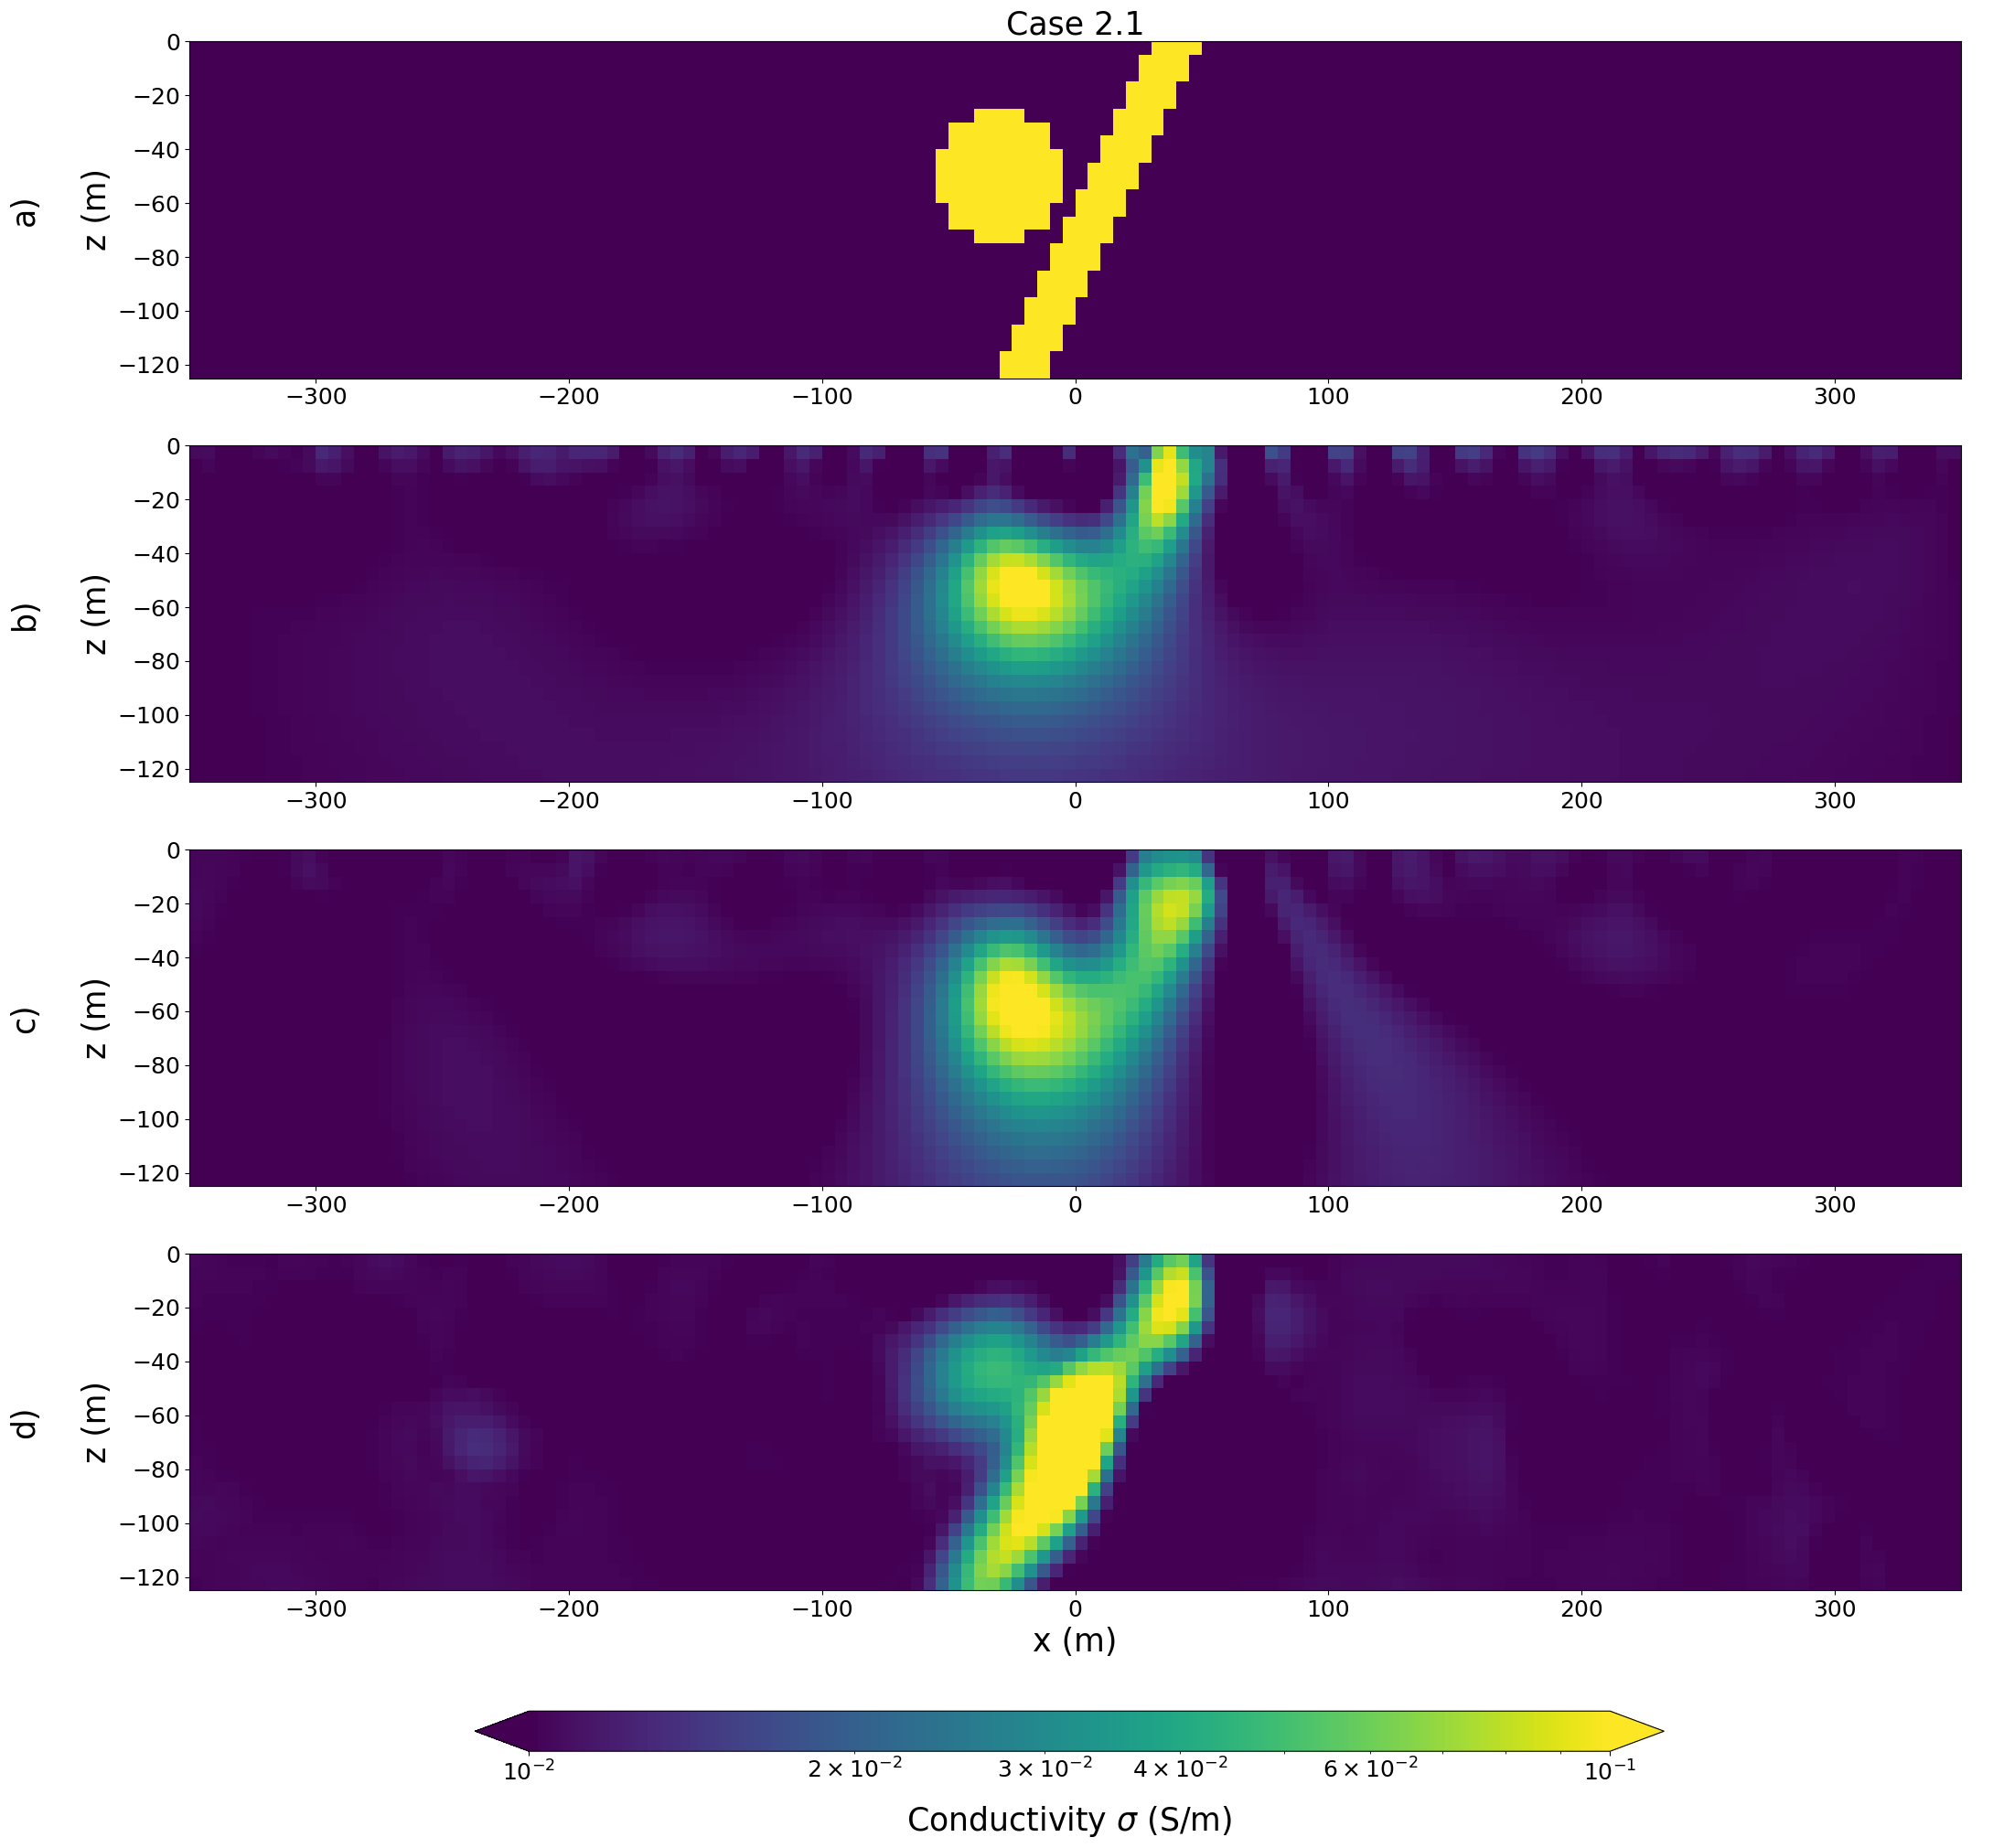
\includegraphics[width=.45\linewidth]{Figure_7_0.03.png}
\caption{(a) is the true model. (b) and (c) are from the conventional sparse-norms inversions without/with sensitivity weighting respectively. (d) is the DIP-Inv result. All inversions are done in the scenario that the observations have 3$\%$ Gaussian noise.}
\label{fig_5}
\end{figure} 

\begin{figure}[h!]
\centering
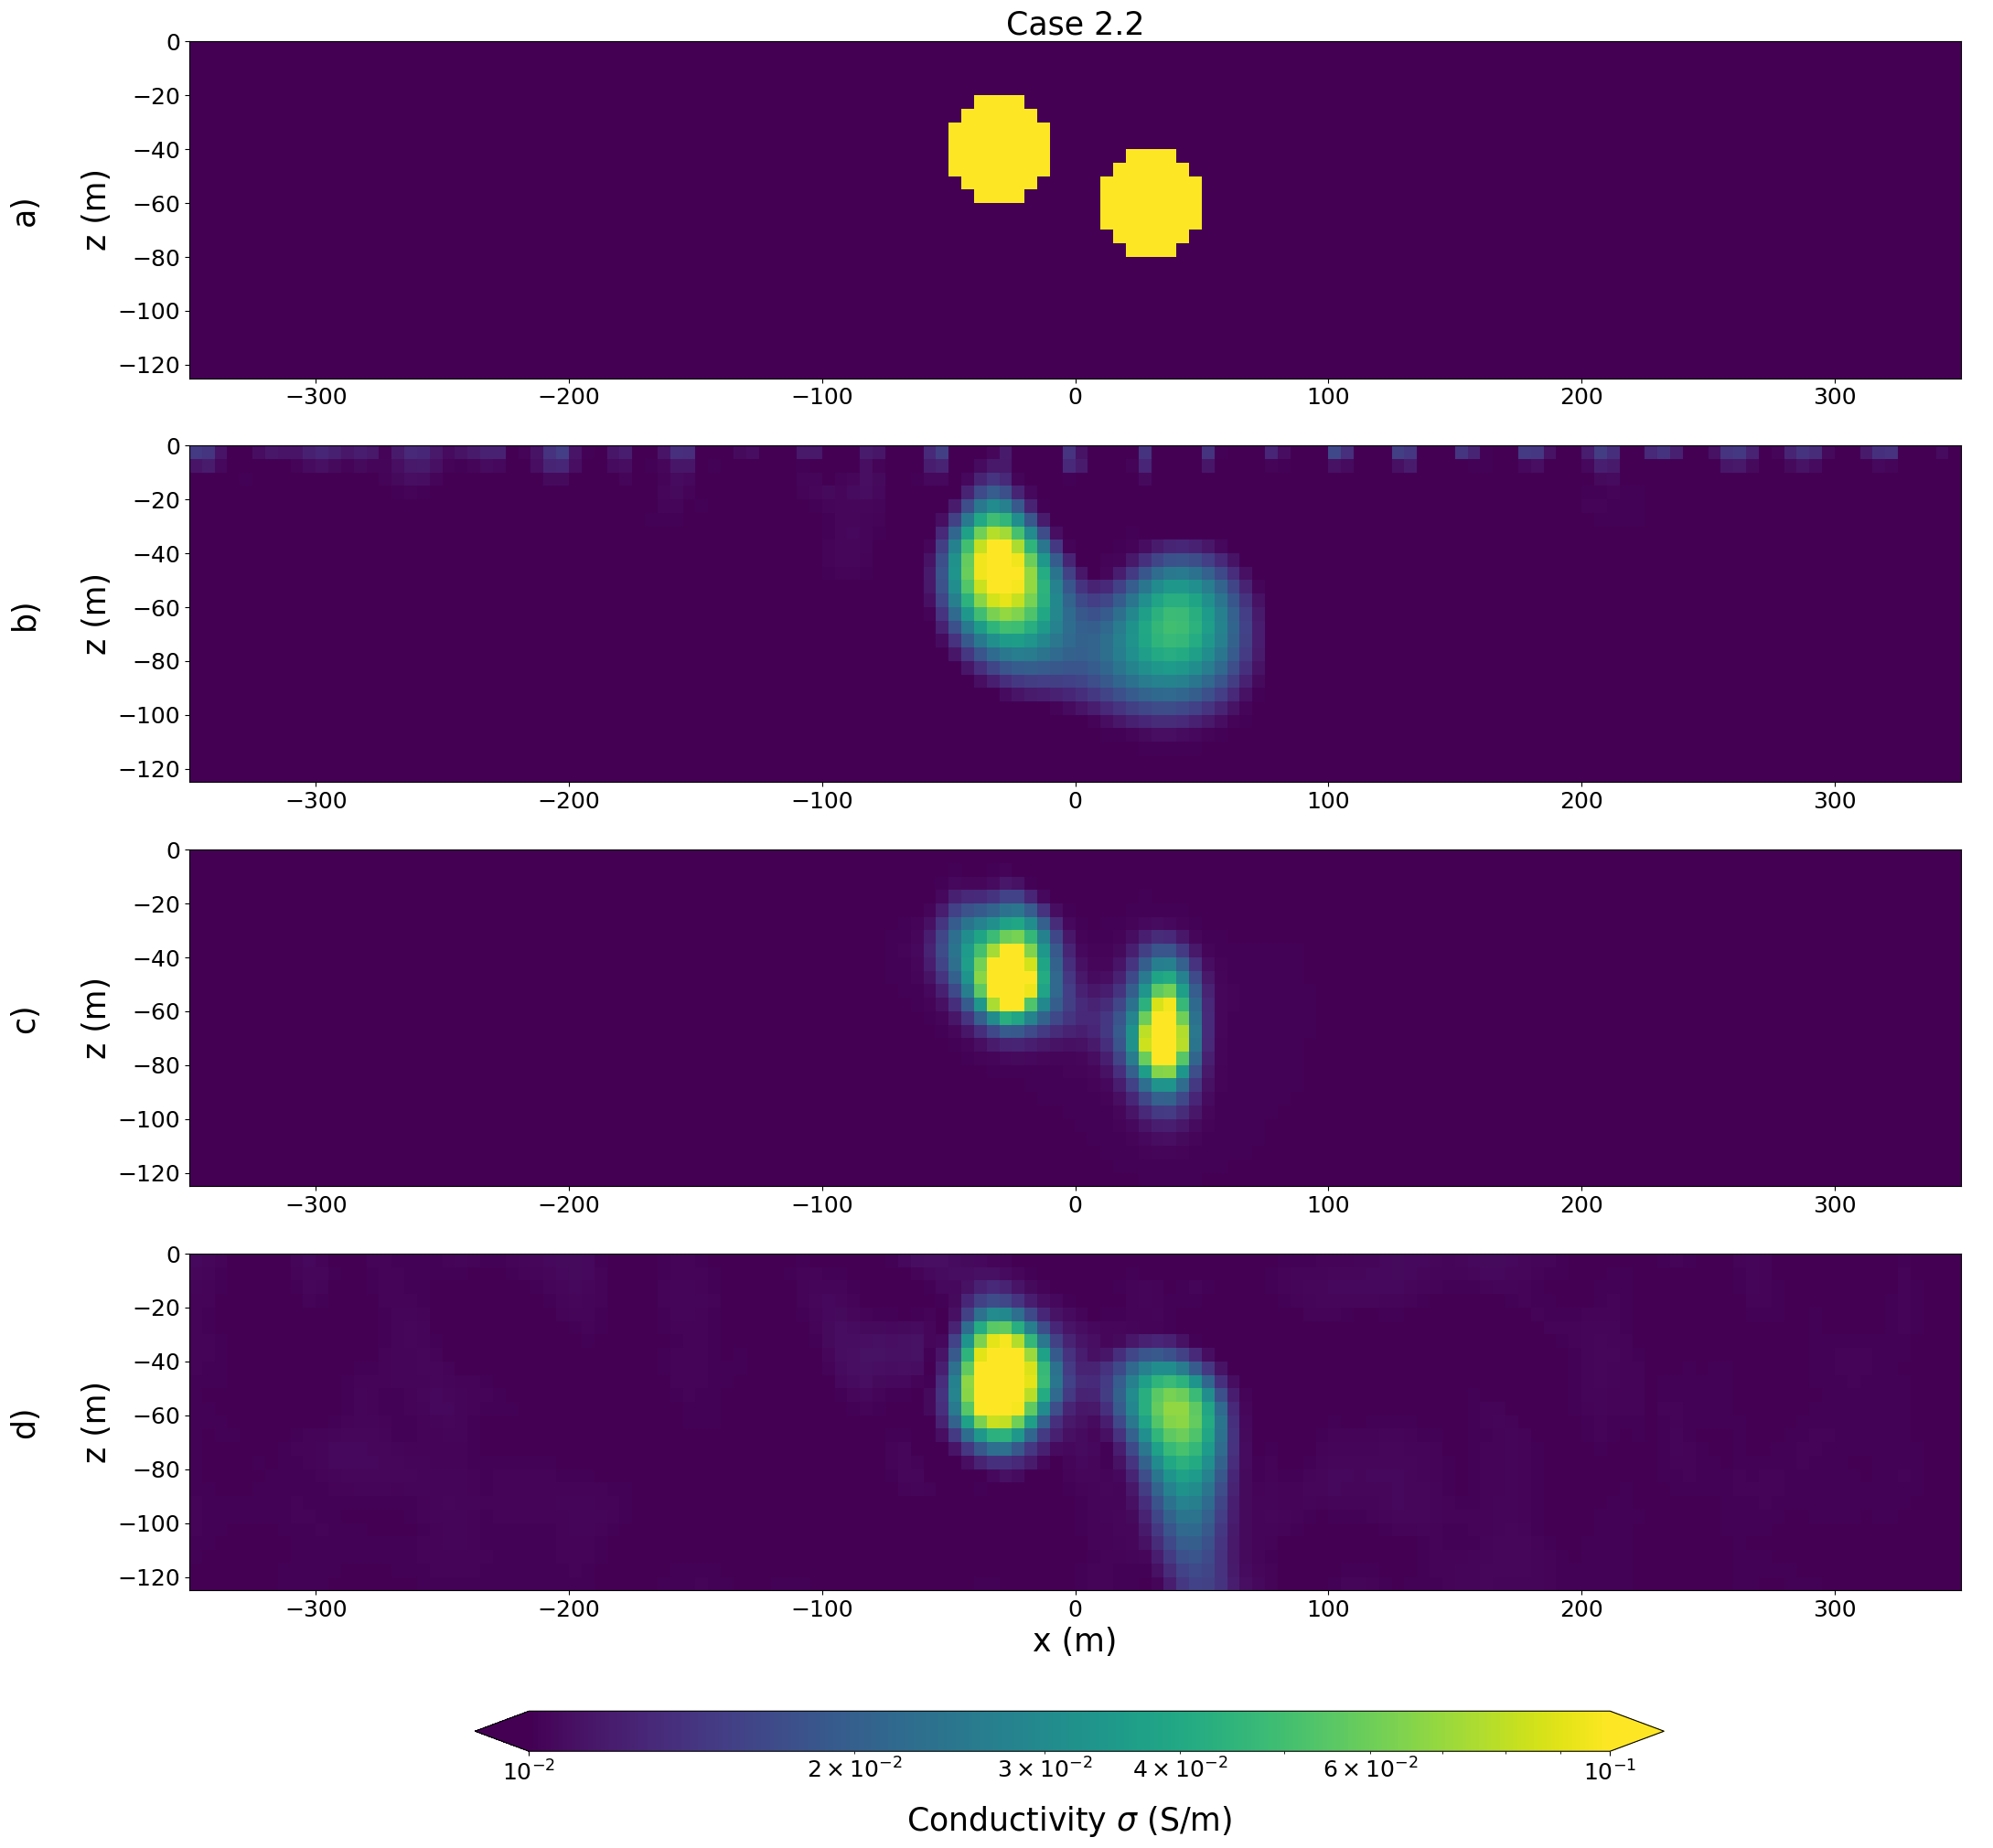
\includegraphics[width=.45\linewidth]{Figure_8_0.03.png}
\caption{(a) is the true model. (b) and (c) are from the conventional sparse-norms inversions without/with sensitivity weighting respectively. (d) is the DIP-Inv result. All inversions are done in the scenario that the observations have 3$\%$ Gaussian noise.}
\label{fig_6}
\end{figure}

\begin{table}[h!]
\centering
\caption{Comparison of DIP-Inv and the conventional method with sensitivity weighting in the scenarios of 3$\%$ noise}
\begin{tabular}{|c|c|l|l|}
\hline
Model & Metrics & Conventional method& DIP-Inv\\
\hline
Case 2.1 & MAE $\downarrow$ & 0.1538 & \textbf{0.0963}\\
 & MSE $\downarrow$ & 0.0045 & \textbf{0.0043}\\
\hline
Case 2.2 & MAE $\downarrow$ & \textbf{0.0385} & 0.0564\\
 & MSE $\downarrow$ & \textbf{0.0028} & 0.0029\\
\hline
\end{tabular}
\label{table:4}
\end{table}

\pagebreak

We choose to show the inversion results with 5$\%$ Gaussian noise since it's a common choice in testing a new algorithm in DCR inversion \cite{1} partly because this noisy level is most common in the industrial cases. Note that the tolerance of the noise level depends not only on the survey method but also on the contrast of conductivity between the anomalies and the host rocks. For example, if the contrast is high, the inversion may have a higher tolerance of the noise level. 

% \section{Results comparison for Case 2}
% We present the MAE and MSE scores here for Case 2.1 and Case 2.2.

% \begin{table}[h!]
% \centering
% \caption{Comparison of the proposed method and the conventional method with sensitivity weighting}
% \begin{tabular}{|c|c|l|l|}
% \hline
% Model & Metrics & Conventional method& DIP-Inv\\
% \hline
% Case 2.1 & MAE $\downarrow$ & 0.1313 & \textbf{0.0997}\\
%  & MSE $\downarrow$ & \textbf{0.0043} & 0.0047\\
% \hline
% Case 2.2 & MAE $\downarrow$ & \textbf{0.0533} & 0.0580\\
%  & MSE $\downarrow$ & 0.0039 & \textbf{0.0033}\\
% \hline
% \end{tabular}
% \label{table:1}
% \end{table}

\bibliographystyle{IEEEtran}
\bibliography{sample}

\end{document}